\chapter{Formati di scambio}
\section{Perchè usarli?}
Nei sistemi distributii, le diverse componenenti sono spesso sviluppate in linguaggi di programmazione differenti e vengono eseguite su sistemi operativi o piattaforme eterogenee.

Poichè questi sistemi non divididono la stessa memoria fisica, i dati devono necessariamente viaggiare sulla rete sotto forma di un flusso ininterrotto di byte.

    \begin{figure}[H]
        \centering
        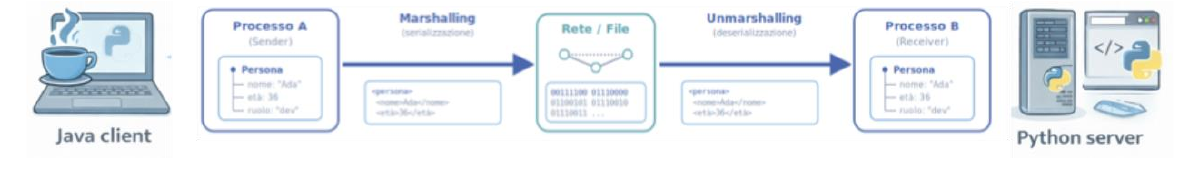
\includegraphics[scale=0.5]{figures/Schermata_20260508_111212.png}
        \caption{Procedura di comunicazione tra client e server attraverso formati di scambio}
    \end{figure}

\section{Come usarli?}
Per far si che sistemi che non si conoscono posasno comunicare e capirsi, è fondamentale concordare un "contratto" comune, \uline{ovvero un formato di scambio dei dati che sia totalmente indipendente dalla piattaforma utilizzata}, come ad esempio i formati di testo \texttt{XML} o \texttt{JSON}.

Per trasferire attraverso la rete delle strutture dati complesse in modo sicuro, le applicazioni si avvolgono di due operazioni speculari:

\subsection{Marshaling (o Serializzazione)}
È il processo mediante il quale l'applicazione \textbf{mittente} \uline{converte le proprie strutture dati residenti in memroia in un formato trasmissible (come testo o byte)} per poi inviarlo sulla rete o salvarlo su un file.

\subsection{Unmarshaling (o Deserializzazione)}
È il processo inverso eseguito dal \textbf{destinatario}.
Ricevuto il flusso di dati serializzato, \uline{il sistema ricevente lo "decompacchetta" e ricostruisce in memoria la struttura dati logica originale} per poterla elaborare correttamente.

\chapter{Linguaggi di Markup}
\section{Definizione}
Sono sistemi di annotazione che usano speciali etichette (tag) per descrivere in modo esplicito la semantica e la struttura dei documenti.

\section{Tipi di marcatura}
Esistono 3 tipologie principali di marcatura:
    
    \begin{itemize}
        \item \textbf{Descrittive}

        Etichettano semplicemnte parti del testo, disaccoppiando la struttura dalla presentazione del testo stesso.

        \item \textbf{Procedurali}

        Definiscono istruzioni per programmi che elaborino il testo al quale sono associate.

        \item \textbf{Presentazione}

        Definiscono come visualizzare il testo al quale sono associate.
    \end{itemize}

\chapter{\texttt{HTML} - HyperText Markup Language}
\section{Definizione}
L'\texttt{HTML} è un linguaggio di marcatura basato su etichette che servono ad annotare un documento in modo che queste annotazioni siano sintatticamente distinguibili dal testo vero e proprio.

\section{Cosa fa?}
Lo scopo principale dell'\texttt{HTML} è quello di \uline{fornire la struttura logica e descrivere la semantica} dei contenuti presenti in una pagina Web.

Il suo ruolo all'interno dell'ecosistema Web è strettamente legato al concetto di \textbf{separazione delle responsabilità}, l'\texttt{HTML} ha il compito esclusivo di \uline{strutturare gerarchicamente l'informazione}, garantendo la totale separazione tra il contenuto e la sua presentazione, la quale viene delegata a \texttt{CSS}.

\begin{figure}[H]
    \centering
    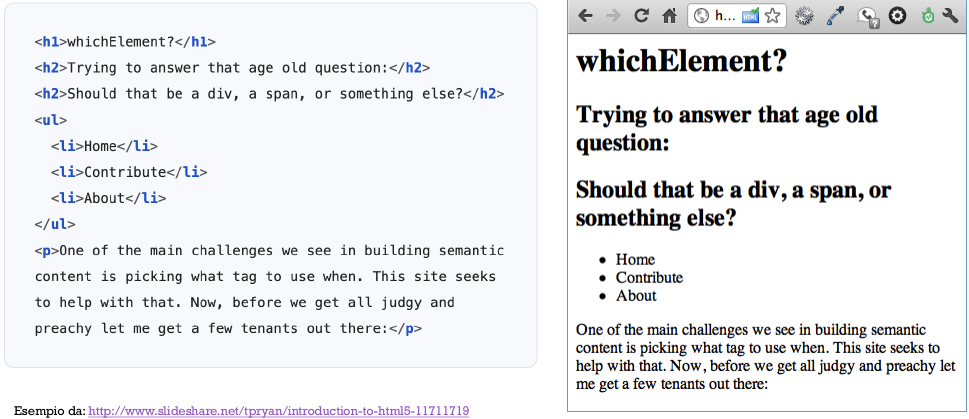
\includegraphics[scale=0.6]{figures/Schermata_20260508_115751.png}
    \caption{Esempio di codice \texttt{HTML} e il suo risultato}
\end{figure}

\newpage

\section{Uso dei Tag e la semantica}
L'\texttt{HTML} struttura il documento racchiudendo le parti di testo all'interno di specifiche etichette di apertura e chiusura.

L'uso corretto di questi tag conferisce un significato preciso al testo contenuto

\begin{table}[htbp]
    \centering
    \renewcommand{\arraystretch}{1.5} % Aumenta un po' lo spazio tra le righe per leggibilità
    
    \begin{tabularx}{\textwidth}{|l|X|}
        \hline
        \textbf{Tag} & \textbf{Significato} \\ \hline
        
        \textless h1\textgreater--\textless h6\textgreater & Intestazioni gerarchiche \\ \hline
        
        \textless p\textgreater & Paragrafo \\ \hline
        
        \textless ul\textgreater, \textless ol\textgreater, \textless li\textgreater & Liste (non ordinata, ordinata, elemento) \\ \hline
        
        \textless table\textgreater & Dati tabulari \\ \hline
        
        \textless form\textgreater, \textless input\textgreater & Form interattivi \\ \hline
        
        \textless a\textgreater & Collegamento ipertestuale \\ \hline
        
        \textless em\textgreater, \textless strong\textgreater & Enfasi semantica \\ \hline
        
        \multicolumn{2}{|p{\dimexpr\textwidth-2\tabcolsep-2\arrayrulewidth}|}{
            \small \textbf{\textless em\textgreater} e \textbf{\textless strong\textgreater} sono semantici (significano \emph{enfasi} e \textbf{importanza}), a differenza di \textbf{\textless i\textgreater} e \textbf{\textless b\textgreater} che sono solo visivi (corsivo e grassetto senza significato).
        } \\ \hline
    \end{tabularx}
\end{table}

\newpage

\section{Interazione con l'utente: Forum}
Quando è necessario richiedere dati all'utente, l'\texttt{HTML} utilizza una struttura specifica chiamata forma, definita dal tag \texttt{<form>}.

All'interno del form, l'\texttt{HTML} mette a disposizione svariati widget di interfaccia, come caselle di testo, checkbox, bottoni e menuù a tendina

Una volta raccolti i dati, il form li invia a uno script lato server (il cui indirizzo è specificato nell'attributo \texttt{action}).
L'invio (definito dall'attributo \texttt{method}) avviene principalmente in 2 modalità:

\begin{itemize}
    \item \textbf{Metodo \texttt{GET}}

    Accoda i parametri inseriti dall'utente direttamente alla fine dell'\texttt{URL} della pagina.

    \item \textbf{Metodo \texttt{POST}}

    Inserisce i dati in modo invisibile all'interno del corpo della richiesta \texttt{HTTP}.
\end{itemize}

\noindent % Evita il rientro della prima riga
\begin{minipage}[t]{0.48\textwidth}
    % --- PRIMA COLONNA: CODICE ---
    \vspace{0pt} % Trucco per allineare correttamente in alto
    \begin{tcolorbox}[title=Esempio codice di un form]
        \begin{lstlisting}[language=HTML, breaklines=true]
<!DOCTYPE html>
<html>
<body>

<h2>HTML Forms</h2>

<form action="/action_page.php">
  <label for="fname">First name:</label><br>
  <input type="text" id="fname" name="fname" value="John"><br>
  <label for="lname">Last name:</label><br>
  <input type="text" id="lname" name="lname" value="Doe"><br><br>
  <input type="submit" value="Submit">
</form>

<p>If you click the "Submit" button...</p>

</body>
</html>
        \end{lstlisting}
    \end{tcolorbox}
\end{minipage}%
\hfill % Crea uno spazio vuoto flessibile tra le due minipage
\begin{minipage}[t]{0.48\textwidth}
    % --- SECONDA COLONNA: IMMAGINE ---
    \vspace{0pt} % Trucco per allineare correttamente in alto
    \centering
    % width=\textwidth si riferisce alla larghezza della minipage, non della pagina intera
    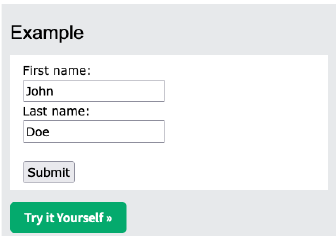
\includegraphics[width=\textwidth]{figures/Schermata_20260508_121814.png}
\end{minipage}

\newpage

\section{\texttt{DOM} - Document Object Model}
\textbf{\texttt{DOM}} è un interfaccia neutrale rispetto al linguaggio di programmazione e alla piattaforma utilizzata, per consentire ai programmi l'accesso e la modifica dinamica di contenuta, strutturura e sile di un documento Web

\subsection{Struttura ad Albero}
Quando il browser riceve la pagina \texttt{HTML}, non la lascia sotto forma di testa, ma la converte in una compleassa \uline{struttura ad albero di oggetti}.

All'interno di questo albero, \uline{ogni singolo tag \texttt{HTML} si trasforma in un "nodo"}, stabilendo cosi' delle \textbf{relazioni gerarchiche di parentela}.

\begin{figure}[H]
    \centering
    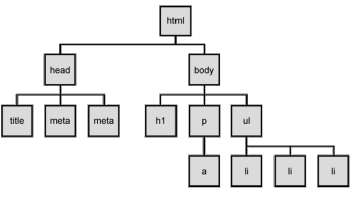
\includegraphics{figures/Albero Dom.png}
    \caption{Esenmpio di albero DOM}
\end{figure}

\subsection{Navigazione dei nodi}
Per permettere ai linguaggi di scripting di muoversi agilmente all'interno di questa architettura, il \texttt{DOM} mette a disposizione diverse proprietà specifiche:

\begin{itemize}
    \item \textbf{\texttt{parentNode}}: Raggiunge il nodo genitore diretto.
    \item \textbf{\texttt{childNodes}}: Restituisce la lista di tutti i nodi figli.
    \item \textbf{\texttt{firstChild}} e \textbf{\texttt{lastChild}}: Puntano rispettivamente al primo e all'ultimo figlio del nodo.
    \item \textbf{\texttt{nextSibling}} e \textbf{\texttt{previousSibling}}: Permettono di spostarsi orizzontalmente sul nodo fratello successivo o su quello precedente.
\end{itemize}

\subsection{Identificazione dei Nodi}
Prima di poter manipolare un elemento della pagina, è necessario "trovarlo" all'interno dell'albero.

Ogni nodo può essere caratterizzato da attributi utili a questo scopo:

\begin{itemize}
    \item Un \textbf{identificatore univoco (ID)}, anche se il \texttt{DOM} non ne garantisce l'assoluta unicità a livello tecnico
    \item Una \textbf{classe}, che indica l'appartenenza a un gruppo specifico
\end{itemize}

\subsection{Funzioni di ricerca per i nodi}
Per sfruttare questi attributi, il browser stesso fornisce nativamente delle funzioni di ricerca rapida, tra cui le più importanti sono:

\begin{itemize}
    \item \textbf{\texttt{getElementById(idName)}}: per estrarre il singolo nodo associato a quel preciso \texttt{ID}.
    \item \textbf{\texttt{getElementiByClassName(ClassName)}}: per estrarre tutti i nodi associati a una specifica classe.
\end{itemize}

\subsection{Eventi e Listener}
Il \texttt{DOM} non serve solo a modificare passivamente la pagina, ma anche a farla reagire alle azioni dell'utente.

Questo avviene tramite gli \textbf{eventi}, ovvero dei segnali emessi dal sistema quando accade qualcosa nel documento.

\texttt{Javascript} può mettersi in ascolto di questi eventi e reagire di conseguenza agganciato delle funzioni specifiche chiamate \textbf{\texttt{listener}}.

\begin{table}[htbp]
    \centering
    \renewcommand{\arraystretch}{1.5} % Migliora la spaziatura verticale delle righe
    
    \begin{tabularx}{\textwidth}{|l|X|}
        \hline
        \textbf{Categoria} & \textbf{Eventi principali} \\ \hline
        \textbf{Mouse} & click, dblclick, mouseover, mouseout \\ \hline
        \textbf{Tastiera} & keydown, keyup, keypress \\ \hline
        \textbf{Form} & submit, change, focus, blur, input \\ \hline
        \textbf{Documento} & DOMContentLoaded, load, resize, scroll \\ \hline
        \textbf{Touch} & touchstart, touchend, touchmove \\ \hline
    \end{tabularx}
\end{table}

\begin{lstlisting}[title=Esempio di codice]
// Seleziono un elemento
const btn = document.getElementById("myBtn");

// Aggiungo un listener
btn.addEventListener("click",function(e)){
    console.log("cliccato", e.target);
}
    
\end{lstlisting}

\chapter{\texttt{CSS} - Cascade Style Sheet}
\section{Definizione}
Il \texttt{CSS} è il linguaggio utilizzato per definire lo stile e la presentazione visiva dei contenuti web.

Il suo obiettivo primario è concretizzare il principio di "separation of concerns" garantendo una netta divisione tra il \textbf{contenuto} e la \textbf{vesta estetica}

\section{Modalità di inclusione}
Il codice \texttt{CSS} può essere applicato a un documento \texttt{HTML} i 3 modi differenzi:
\begin{itemize}
    \item \textbf{Inline}

    Inserito direttamente sul singolo tag \texttt{HTML} tramite l'attributi \texttt{style=""}.

    \item \textbf{Interno}

    Definito all'interno di un blocco di tag \texttt{<style>} situato nella sezione \texttt{<head>} della pagina.

    \item \textbf{Esterno}

    Scritto all'interno di un file \texttt{.css} separato e collegato alla pagina \texttt{HTML} tramite il tag \texttt{<link rel="stylesheet" href="theme.css"}.

    Questo è il modello preferito perchè \uline{separa fisicamente contenuto e stile}.
\end{itemize}

\newpage

\section{Struttura Base}
Una regola \texttt{CSS} è composta da un "selettore" seguito da un blocco di dichiarazione racchiuse tra parentesi graffe.

Ogni dichiarazione è una coppia proprità/valore (\texttt{selettore{proprietà: valore;}})

\begin{tcolorbox}[title=Esempio codice CSS]
    \begin{lstlisting}
h1{
    color: red;
    font-size: 2em;
}
    \end{lstlisting}
\end{tcolorbox}

\subsection{Selettori}
I selettori sono il meccanismo con cui il \texttt{CSS} individua precisi elementi o gruppi di elementi nell'albero \texttt{DOM} a cui applicare il design.

\subsubsection{Selettori fondamentali}
\begin{itemize}
    \item \textbf{Elemento (Tag)}: Seleziona tutti gli elementi di un certo tipo.
    \item \textbf{Classe}: Individua gli elementi che possiedono uno specifico attributo \texttt{class}, preceduto da un punto.
    \item \textbf{ID}: Punta a un elemento univoco contrassegnato da uno specifico attributo \texttt{id}, preceduto dal cancelletto.
    \item \textbf{Universale}: L'asterisco (\texttt{*{...}}) permette di selezionare indiscriminatamente tutti gli elementi della pagina
\end{itemize}

\subsection{Combinatori}
I combinatori servono per selezionare elementi non per il tag che sono, ma per la loro posizione all'interno dell'albero \texttt{DOM}
\begin{itemize}
    \item \textbf{Discendente:} \texttt{div p} seleziona tutti i paragrafi contenuti dentro un div.
    \item \textbf{Figlio diretto}: \texttt{ul > li} seleziona esclusivamente gli elementi della lista che sono figli diretti del tag \texttt{ul}
    \item \textbf{Gruppo:} \texttt{h1, h2, h3} consente di raggruppare selettori diversi applicando la stessa regola in un colpo solo
\end{itemize}

\newpage

\subsection{Pseudo-classi}
Un elemento HTML è sempre lo stesso tag, ma a livello di intefraccia può cambiare stato.

Le psuedo classi permettono di stilizzare questi stati dinamicamente, senza alterare l'\texttt{HTML}, esempi notevoli sono:
\begin{itemize}
    \item \textbf{\texttt{a:hover}}
    \item \textbf{\texttt{input:focus}}
    \item \textbf{\texttt{li:first-child}}
\end{itemize}

\section{Algoritmo "a Cascata"}
Poichè esistono diversi fogli di stile, è del tutto normale che le regole si sovrappongano e generino dei conflitti.

Il termine "Cascading" si riferisce all'algoritmo che decide quale regola abbia la precedenza.

La priorit viene valutata secondo quest'ordine:
\begin{enumerate}
    \item \textbf{Importanza}
    
    L'eventuale utilizzo del flag esplicito \texttt{!important} associato a un attributo.
    
    \item \textbf{Specificità}

    Dipende dal settore utilizzato.

    Un ID è più specifico di una classe, che a sua volta prevale sul selettore di un semplice elemento.

    \item \textbf{Ordine nel sorgente}

    A parità di specificità, vince la regola dichiarata per ultima nel file.
\end{enumerate}

\section{Media Query}
Per far si' che la grafica si adatti ai diversi dispositivi, si utilizzano le "media query".

Questi costrutti \texttt{CSS} applicano stili in modo condizionale verificando le caratteristiche del dispositivo in uso, come la larghezza, l'altezza, la risoluzione e l'orientamento dello schemro.

Ad esempio, \texttt{@media screen and (min-width: 480px)}

\chapter{XML - eXtensible Markup Language}